% This file was created by matlab2tikz.
% Minimal pgfplots version: 1.9
%
%The latest updates can be retrieved from
%  http://www.mathworks.com/matlabcentral/fileexchange/22022-matlab2tikz
%where you can also make suggestions and rate matlab2tikz.
%
\begin{figure}[!htbp]
\centering
\begin{minipage}[l]{\textwidth}
\resizebox{90mm}{80mm} 
{
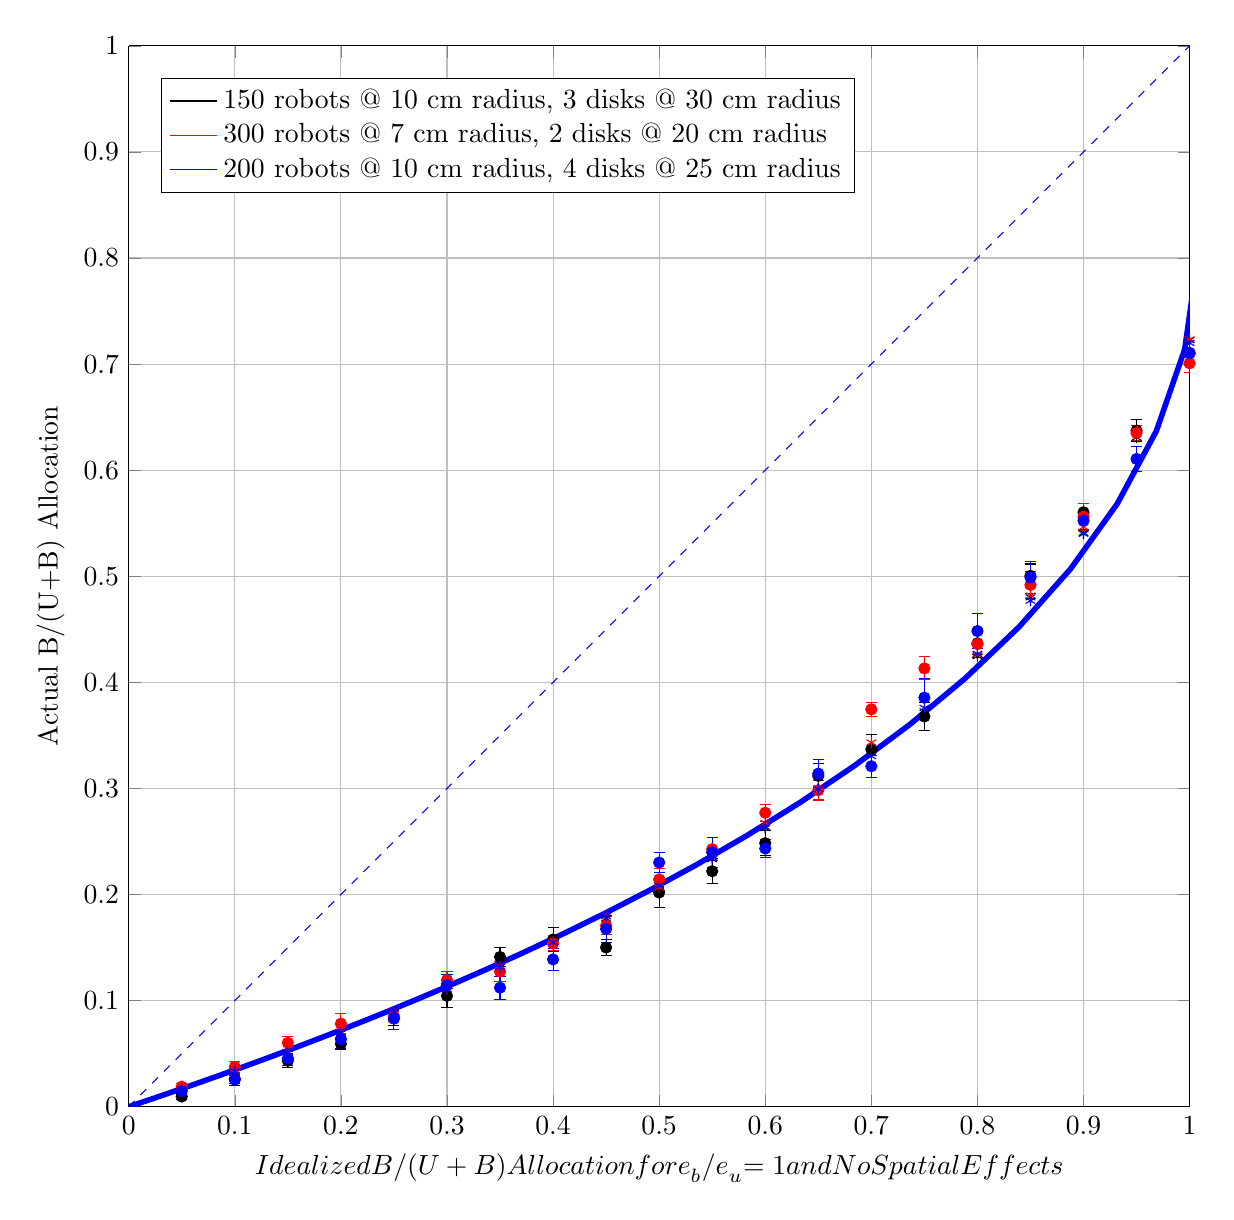
\begin{tikzpicture}
\begin{axis}[%
width=5.304444in,
height=5.304444in,
at={(0.889778in,0.774778in)},
scale only axis,
separate axis lines,
every outer x axis line/.append style={black},
every x tick label/.append style={font=\color{black}},
xmin=0,
xmax=1,
xlabel={$\text{Idealized B/(U+B) Allocation for e}_\text{b}\text{/e}_\text{u}\text{=1 and No Spatial Effects}$},
xmajorgrids,
every outer y axis line/.append style={black},
every y tick label/.append style={font=\color{black}},
ymin=0,
ymax=1,
ylabel={Actual B/(U+B) Allocation},
ymajorgrids,
legend style={at={(0.03,0.97)},anchor=north west,legend cell align=left,align=left,draw=black}
]
\addplot [color=black,solid]
  table[row sep=crcr]{%
0	0\\
};
\addlegendentry{150 robots @ 10 cm radius, 3 disks @ 30 cm radius};

\addplot [color=red,solid]
  table[row sep=crcr]{%
0	0\\
};
\addlegendentry{300 robots @ 7 cm radius, 2 disks @ 20 cm radius};

\addplot [color=blue,solid]
  table[row sep=crcr]{%
0	0\\
};
\addlegendentry{200 robots @ 10 cm radius, 4 disks @ 25 cm radius};

\addplot [color=black,only marks,mark=asterisk,mark options={solid},forget plot]
  table[row sep=crcr]{%
0.05	0.0162597936433945\\
0.1	0.0331519099766532\\
0.15	0.0506946151920453\\
0.2	0.0692469094010075\\
0.25	0.0885400505925061\\
0.3	0.109332036369888\\
0.35	0.131654234305656\\
0.4	0.1548347890559\\
0.45	0.17740871791421\\
0.5	0.20501056014977\\
0.55	0.233348748138753\\
0.6	0.262591203061691\\
0.65	0.299975714656033\\
0.7	0.333558200946357\\
0.75	0.372691885449244\\
0.8	0.424682014198157\\
0.85	0.480138096604043\\
0.9	0.540990976026119\\
0.95	0.630723096084231\\
1	0.722543728572875\\
};
\addplot [color=black,only marks,mark=*,mark options={solid},forget plot]
 plot [error bars/.cd, y dir = both, y explicit]
 table[row sep=crcr, y error plus index=2, y error minus index=3]{%
0.05	0.00959805437511649	0.00311090845175374	0.00311090845175374\\
0.1	0.0261935729734324	0.00628501646367648	0.00628501646367648\\
0.15	0.0433789161422863	0.00630110231265376	0.00630110231265376\\
0.2	0.0593041795468092	0.00575289837076141	0.00575289837076141\\
0.25	0.0846130156644347	0.00806004405597278	0.00806004405597278\\
0.3	0.104479379608461	0.0113323343896263	0.0113323343896263\\
0.35	0.141102123397313	0.00912642032209818	0.00912642032209818\\
0.4	0.157590401164622	0.0115041723613989	0.0115041723613989\\
0.45	0.150056732786388	0.00777825176260621	0.00777825176260621\\
0.5	0.201907674578219	0.0140885848991427	0.0140885848991427\\
0.55	0.221961709976507	0.0118506947890386	0.0118506947890386\\
0.6	0.248396574819705	0.0119984291597447	0.0119984291597447\\
0.65	0.311856336568031	0.0114628610113	0.0114628610113\\
0.7	0.336816639984884	0.0142966576283983	0.0142966576283983\\
0.75	0.367836050353627	0.0130610326639296	0.0130610326639296\\
0.8	0.436765094483304	0.0137267478231265	0.0137267478231265\\
0.85	0.500439337893644	0.0110925882354466	0.0110925882354466\\
0.9	0.560333342010991	0.00851826116025256	0.00851826116025256\\
0.95	0.637278638258434	0.0106480749052953	0.0106480749052953\\
1	0.710470505420636	0.0121552750022706	0.0121552750022706\\
};
\addplot [color=red,only marks,mark=asterisk,mark options={solid},forget plot]
  table[row sep=crcr]{%
0.05	0.0163157916936749\\
0.1	0.0333889167251306\\
0.15	0.0513358575649547\\
0.2	0.070132917627186\\
0.25	0.0893883037603915\\
0.3	0.11079087415269\\
0.35	0.132247342763885\\
0.4	0.155651833643117\\
0.45	0.179853816805476\\
0.5	0.206632831247039\\
0.55	0.235112681911031\\
0.6	0.267534627300878\\
0.65	0.299334510861068\\
0.7	0.343320332984026\\
0.75	0.384880173220095\\
0.8	0.42620886711763\\
0.85	0.481854990137991\\
0.9	0.546468153956028\\
0.95	0.636651350699871\\
1	0.723330692960006\\
};
\addplot [color=red,only marks,mark=*,mark options={solid},forget plot]
 plot [error bars/.cd, y dir = both, y explicit]
 table[row sep=crcr, y error plus index=2, y error minus index=3]{%
0.05	0.0188624240313818	0.00321468702820613	0.00321468702820613\\
0.1	0.0374825042850584	0.00507061060729123	0.00507061060729123\\
0.15	0.0602022334449133	0.00621473785569926	0.00621473785569926\\
0.2	0.0782366495691359	0.00943837591680487	0.00943837591680487\\
0.25	0.0851636425485405	0.00433560062346917	0.00433560062346917\\
0.3	0.11937450583458	0.00830769621775972	0.00830769621775972\\
0.35	0.127392045813658	0.00918105063256683	0.00918105063256683\\
0.4	0.153868103527942	0.00650885732985215	0.00650885732985215\\
0.45	0.170710996078448	0.00820470410760432	0.00820470410760432\\
0.5	0.214191508861708	0.0105017017872699	0.0105017017872699\\
0.55	0.242727488686486	0.010637368607121	0.010637368607121\\
0.6	0.277059523861378	0.00802044468430474	0.00802044468430474\\
0.65	0.298304995040193	0.00920720573105538	0.00920720573105538\\
0.7	0.374582699072879	0.00670666914607881	0.00670666914607881\\
0.75	0.413175945672419	0.0109011246450817	0.0109011246450817\\
0.8	0.435996651406318	0.0100084692128696	0.0100084692128696\\
0.85	0.491877087482157	0.0130264981445514	0.0130264981445513\\
0.9	0.556057797944396	0.0126568835558961	0.0126568835558961\\
0.95	0.635041674161455	0.00674993969912019	0.00674993969912019\\
1	0.700777423863967	0.00854166059682437	0.00854166059682437\\
};
\addplot [color=blue,only marks,mark=asterisk,mark options={solid},forget plot]
  table[row sep=crcr]{%
0.05	0.0163110620635054\\
0.1	0.0333189025282509\\
0.15	0.0511317945559411\\
0.2	0.0699039401441017\\
0.25	0.08938146620515\\
0.3	0.110678086595137\\
0.35	0.131547684905416\\
0.4	0.15487548454289\\
0.45	0.179430591313944\\
0.5	0.208518277746576\\
0.55	0.234834330030575\\
0.6	0.263646405657964\\
0.65	0.299158420803768\\
0.7	0.330425930542452\\
0.75	0.375920471775434\\
0.8	0.426967884738187\\
0.85	0.476937672326827\\
0.9	0.539986629430774\\
0.95	0.610224733607538\\
1	0.719948277904586\\
};
\addplot [color=blue,only marks,mark=*,mark options={solid},forget plot]
 plot [error bars/.cd, y dir = both, y explicit]
 table[row sep=crcr, y error plus index=2, y error minus index=3]{%
0.05	0.0146647021458012	0.00304554907186302	0.00304554907186302\\
0.1	0.0254249657747958	0.0039143778655929	0.0039143778655929\\
0.15	0.0455005433454628	0.00674369033715434	0.00674369033715434\\
0.2	0.0635777862421737	0.00851101500529636	0.00851101500529636\\
0.25	0.0829462607743639	0.00986522383089683	0.00986522383089683\\
0.3	0.114550692233239	0.00973614540210394	0.00973614540210394\\
0.35	0.112183434234861	0.0107831213809295	0.0107831213809295\\
0.4	0.138838144424399	0.0101293548048703	0.0101293548048703\\
0.45	0.167583420118998	0.0127010309698205	0.0127010309698205\\
0.5	0.230177410829379	0.00946162600931111	0.00946162600931111\\
0.55	0.239707930043631	0.0141735157109557	0.0141735157109557\\
0.6	0.243427906898226	0.00849075465541432	0.00849075465541432\\
0.65	0.313984492694062	0.013099892902882	0.013099892902882\\
0.7	0.320932548637356	0.0104023150918056	0.0104023150918056\\
0.75	0.385586361242429	0.0177455594151495	0.0177455594151495\\
0.8	0.448334070004652	0.0167524970495649	0.0167524970495649\\
0.85	0.498876565450558	0.0153727650381449	0.015372765038145\\
0.9	0.552431934712582	0.00872748594585593	0.00872748594585593\\
0.95	0.610568101919522	0.012146644442102	0.012146644442102\\
1	0.710177399513643	0.00851252025065674	0.00851252025065674\\
};
\addplot [color=blue,dashed,forget plot]
  table[row sep=crcr]{%
0	0\\
0.1	0.1\\
0.2	0.2\\
0.3	0.3\\
0.4	0.4\\
0.5	0.5\\
0.6	0.6\\
0.7	0.7\\
0.8	0.8\\
0.9	0.9\\
1	1\\
};
\addplot [color=blue,solid,line width=2.0pt,forget plot]
  table[row sep=crcr]{%
2.9936606163795e-05	1e-05\\
3.35527523533561e-05	1.12079493971978e-05\\
3.76056993430236e-05	1.25618129690145e-05\\
4.21482075487107e-05	1.40792164093777e-05\\
4.72394098320154e-05	1.57799145068502e-05\\
5.29455810684167e-05	1.76860483284884e-05\\
5.93410006264883e-05	1.98224334702092e-05\\
6.65089189687773e-05	2.22168831263423e-05\\
7.45426409359732e-05	2.49005701843501e-05\\
8.35467397893457e-05	2.79084330587567e-05\\
9.36384177815432e-05	3.12796305477627e-05\\
0.000104949030924437	3.50580516342365e-05\\
0.000117625797748983	3.92928868680868e-05\\
0.000131833714233176	4.40392687687333e-05\\
0.000147757699740312	4.93589895849556e-05\\
0.00016560500179475	5.53213057564993e-05\\
0.000185607890863864	6.20038395505749e-05\\
0.000208026680054892	6.94935896114812e-05\\
0.000233153108820822	7.78880635795108e-05\\
0.000261314134452381	8.72965475244879e-05\\
0.000292876180371759	9.78415287204529e-05\\
0.000328249896102341	0.000109660290284331\\
0.000367895490339156	0.000122906698438879\\
0.000412328705866486	0.00013775320566796\\
0.000462127513250081	0.000154393095842827\\
0.000517939609369235	0.000173043000548311\\
0.000580490817055915	0.000193945719368474\\
0.000650594493492838	0.000217373380848497\\
0.000729162067719828	0.000243630985284775\\
0.00081721484175084	0.000273060375466118\\
0.000915897205568287	0.000306044687060407\\
0.00102649143380653	0.000343013336585427\\
0.00115043425144606	0.000384447611901342\\
0.00128933537751211	0.000430886938006377\\
0.00144499827981734	0.000482935899708895\\
0.00161944340043346	0.000541272112602747\\
0.00181493414105607	0.000606655044816591\\
0.00203400592998685	0.000679935904385909\\
0.0022794987283459	0.000762068720969516\\
0.00255459337259517	0.000854122766181355\\
0.00286285219374022	0.000957296474235519\\
0.00320826440090582	0.00107293304413475\\
0.00359529676853592	0.00120253792652436\\
0.00402895022238924	0.00134779842286962\\
0.00451482297984206	0.00151060565211456\\
0.00505918096472178	0.00169307917080209\\
0.00566903628577086	0.00189759456717994\\
0.00635223464047479	0.00212681438853501\\
0.00711755258169445	0.00238372280439325\\
0.00797480566227983	0.00267166445685859\\
0.00893496855109295	0.00299438800387629\\
0.0100103082905112	0.00335609492230214\\
0.0112145319376125	0.00376149420613547\\
0.0125629498949642	0.00421586367202189\\
0.014072656287084	0.00472511867015056\\
0.015762727768472	0.00529588909508018\\
0.0176544421498792	0.00593560569908301\\
0.0197715181899806	0.0066525968317041\\
0.0221403778055551	0.00745619686496977\\
0.024790431786605	0.00835686771581256\\
0.0277543898408722	0.00936633504779028\\
0.0310685954066577	0.0104977409252833\\
0.0347733851286663	0.0117658149075467\\
0.0389134721456661	0.0131870658100579\\
0.0435383513383976	0.0147799966296645\\
0.0487027233675891	0.0165653454316034\\
0.0544669326184634	0.0185663553344511\\
0.0608974119686026	0.0208090771078921\\
0.0680671245032544	0.023322708322764\\
0.0760559887916838	0.0261399734687142\\
0.0849512699678608	0.0292975499881441\\
0.0948479134693456	0.032836545772899\\
0.105848791705484	0.0368030343401421\\
0.11806482596539	0.0412486546547644\\
0.131614936350355	0.0462312834073084\\
0.146625761245906	0.051815788499662\\
0.163231074682807	0.0580748735480114\\
0.181570814767797	0.065090024397477\\
0.20178961916141	0.0729525699709289\\
0.224034744411895	0.0817648712629699\\
0.248453225020848	0.0916416539583756\\
0.27518810576232	0.102711502024098\\
0.304373557477953	0.115118531719627\\
0.3361286628602	0.129024267819328\\
0.370549635031015	0.144609746472952\\
0.407700207976829	0.162077872081044\\
0.447599912974054	0.181656058868983\\
0.490209925752515	0.203599191549794\\
0.535416128178208	0.228192943620046\\
0.583008962078453	0.255757496489108\\
0.632659537292147	0.28665170786039\\
0.683891250106208	0.321277783631956\\
0.736045804559953	0.360086514139082\\
0.788241898970815	0.403583142908417\\
0.839323769516374	0.452333944327956\\
0.887794993134982	0.50697359586626\\
0.931729993380912	0.568213440818442\\
0.968650830683473	0.636850749150072\\
0.995348886146693	0.713779097004149\\
1.00761800428462	0.8\\
};
\end{axis}
\end{tikzpicture}%
} % resizebox
\end{minipage}
\caption{Effect of varying environmental parameters on robot allocations \cite{PavlicISRR2013}.
        Ten trials were generated for each disk size, and the
        average across the trials are shown with error bars
        indicating $\pm 1$ standard error of the mean. A dashed line of
        unity slope is shown for reference. The solid line represents
        the predicted curve based on the robot collision-avoidance distance $a$, which
        is non\-/zero for these cases.}
        \label{fig:EnvRob}
\end{figure}
